\documentclass[supercite]{Experimental_Report}

\title{\textit{Christoph Rösmann, Wendelin Feiten, Thomas Wösch, Frank Hoffmann, Torsten Bertram,Trajectory modification considering dynamic constraint of autonomous robots,ROBOTIK 2012}}
\school{计算机科学与技术学院}
\author{朱旭鹏}
\classnum{CSXJ1902}
\stunum{U201913821}
\instructor{余辰} % 李平、孙伟平、范晔斌、陈加忠
\usepackage{zhnumber} % change section number to chinese
\usepackage{tikz}
\usetikzlibrary{mindmap,trees}
\usepackage{algorithm, multirow}
\usepackage{algpseudocode}
\usepackage{amsmath}
\usepackage{amsthm}
\usepackage{framed}
\usepackage{mathtools}
\usepackage{subcaption}
\usepackage{amsmath, amssymb, amsfonts}
\usepackage{tabu}
\usepackage{xltxtra} %提供了针对XeTeX的改进并且加入了XeTeX的LOGO, 自动调用xunicode宏包(提供Unicode字符宏)
\usepackage{bm}
\usepackage{longtable}
\usepackage{tikz}
\usepackage{pdfpages}
\usepackage{tikzscale}
\usepackage{pgfplots}
%\usepackage{enumerate}
\usepackage{graphicx}
\pgfplotsset{compat=1.16}

\newcommand{\cfig}[3]{
  \begin{figure}[htb]
    \centering
    \includegraphics[width=#2\textwidth]{images/#1.tikz}
    \caption{#3}
    \label{fig:#1}
  \end{figure}
}

\newcommand{\sfig}[3]{
  \begin{subfigure}[b]{#2\textwidth}
    \includegraphics[width=\textwidth]{images/#1.tikz}
    \caption{#3}
    \label{fig:#1}
  \end{subfigure}
}

\newcommand{\xfig}[3]{
  \begin{figure}[htb]
    \centering
    #3
    \caption{#2}
    \label{fig:#1}
  \end{figure}
}

\newcommand{\rfig}[1]{\autoref{fig:#1}}
\newcommand{\ralg}[1]{\autoref{alg:#1}}
\newcommand{\rthm}[1]{\autoref{thm:#1}}
\newcommand{\rlem}[1]{\autoref{lem:#1}}
\newcommand{\reqn}[1]{\autoref{eqn:#1}}
\newcommand{\rtbl}[1]{\autoref{tbl:#1}}

\algnewcommand\Null{\textsc{null }}
\algnewcommand\algorithmicinput{\textbf{Input:}}
\algnewcommand\Input{\item[\algorithmicinput]}
\algnewcommand\algorithmicoutput{\textbf{Output:}}
\algnewcommand\Output{\item[\algorithmicoutput]}
\algnewcommand\algorithmicbreak{\textbf{break}}
\algnewcommand\Break{\algorithmicbreak}
\algnewcommand\algorithmiccontinue{\textbf{continue}}
\algnewcommand\Continue{\algorithmiccontinue}
\algnewcommand{\LeftCom}[1]{\State $\triangleright$ #1}


\newtheorem{thm}{定理}[section]
\newtheorem{lem}{引理}[section]
\renewcommand {\thefigure} {\arabic{figure}}
\colorlet{shadecolor}{black!15}

\theoremstyle{definition}
\newtheorem{alg}{算法}[section]
\def\thmautorefname~#1\null{定理~#1~\null}
\def\lemautorefname~#1\null{引理~#1~\null}
\def\algautorefname~#1\null{算法~#1~\null}
\usepackage{xcolor}
\usepackage{listings}
\usepackage[skins]{tcolorbox}
\tcbuselibrary{breakable}
\newtcolorbox{abox}[1][]{enhanced,
	fonttitle = \heiti \large \bfseries,% 标题字体设置
	colbacktitle =black,% 标题背景颜色
	coltitle=white,% 标题字体颜色
	% halign title=center,% 标题对齐方式
	attach boxed title to top left = {yshift = -5pt},
	%	将标题以box 形式放在文本框左上角，并向下移动5pt	
	%----------正文字体--------
	fontupper = \kaishu,%正文字体设置
	%colback = white,%正文背景颜色设置
	%---------边框设置---------
	arc = 4pt,%正文边框边角弧度
	%	boxed title style={arc=0pt},%标题框边角弧度
	colframe=black,%边框颜色设置
	toprule  = 1pt,%取消上边框
	rightrule = 1pt,%取消下边框
	%---------调整字体位置------
	top = 10pt,%增大正文文本与上边框距离
	%---------设置标题为默认参数，不影响其他参数的设置
	title=#1,
	breakable
}
\newcommand{\tabincell}[2]{\begin{tabular}{@{}#1@{}}#2\end{tabular}}  
\begin{document}

\maketitle
\clearpage

\pagenumbering{Roman}

\pagenumbering{arabic}

\begin{abstract}
经典的“elastic band”使全局规划器生成的路径相对于最短路径长度发生改变,同时避免与障碍物接触.它不直接考虑底层机器人的任何动态约束.这一篇文章引入了一种称为“Time Elastic Band”的新方法,该方法明确考虑了根据动态约束（例如有限的机器人速度和加速度）的运动.该问题是在加权多目标优化框架中提出的.大多数目标都取决于当地在几个相邻的中间配置上.所以我们使用基于稀疏系统矩阵约束的最小二乘优化方法.

仿真和实际机器人实验的结果表明,该方法具有鲁棒性和计算能力有效地实时生成最佳机器人轨迹.这个方法转换由以下组成的初始路径一系列路线指向一条明显依赖于时间的轨迹,从而实现对机器人的实时控制时间由于其模块化公式,该方法易于扩展,以纳入额外的目标和约束.
\end{abstract}

\section{引入}

假设初始路径已由全局规划器生成\cite{1},则进行局部路径修改.特别是在服务机器人的情况下,由于动态环境的固有不确定性,路径的修改是优选的方法,因为环境可能是动态的.此外,由于局部、不完整的地图和动态观测,环境模型可能会发生变化.此外,大规模全局路径的（重新）计算在实时应用中通常是不可行的.这一观察导致了局部修改路径的方法,如[2,3]提出的“弹性带”.“弹性带”方法的主要思想是将最初给定的路径视为弹性橡胶带,使其变形,该弹性橡胶带在尝试收缩路径的同时保持与障碍物的距离时受到内部和外部力的平衡.

这一观察提出了修改局部路径的方法例如\cite{2} \cite{3} 提出的“elastic band”方法.这个“elastic band”方法的主要思想是使最初给定的路径是将其视为弹性橡胶,这个橡胶受到了外力和内力的约束导致了橡胶形状的变化,也就是路径的变化.

后来,这种方法被扩展到非完整运动学\cite{4} \cite{5} \cite{6},具有许多自由度的机器人系统\cite{7}和具有动力学障碍\cite{8}的系统.
\begin{figure}
\centering
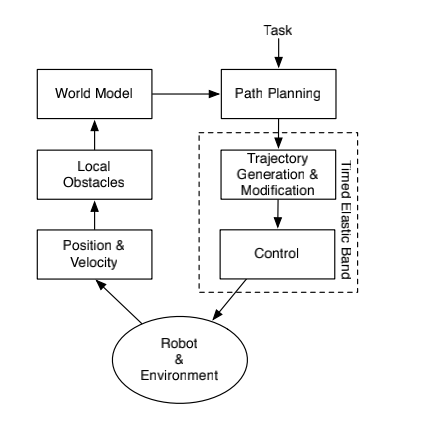
\includegraphics[width=0.3\textwidth]{1.png}
\caption{\label{fig:1}使用TEB算法的机器人系统}
\end{figure}
然而,动态运动约束尚未被认为是局部路径规划的最终目标.我们需要获得可执行的路径,典型的方法是平滑路径,例如使用样条曲线以获得动态可行的轨迹.

我们的方法被称为“TEB”,这是一种新颖的方法,因为它明确地用时间信息增强了“弹性带”的功能,从而允许考虑机器人的动力学约束和直接修改轨迹而不是路径.图\ref{fig:1}显示了带有“定时弹性带”的机器人系统的结构.通过考虑时间信息,“定时弹性带”可以用于控制机器人的速度和加速度.尽管本文考虑了在具有三个全局自由度和两个局部自由度的平面环境中移动的差速驱动移动机器人,但新方法适用于高维状态空间.


\section{TEB算法介绍}

传统的“elastic band”可以表示为一组瞬间的“机器人状态三元组”,形式化表示是$\boldsymbol{x}_i = (x_i,y_i,\beta_i)^T \in \mathcal{R}^2*S^1$,在这个式子里面,$x_i,y_i$表示为机器人的绝对位置,而$\beta_i$可以表示为机器人的偏向角,如图\ref{fig:2}所示.注意,这一组标注的状态集合的三元组是基于一个坐标系的.

\begin{figure}[htbp]
\centering
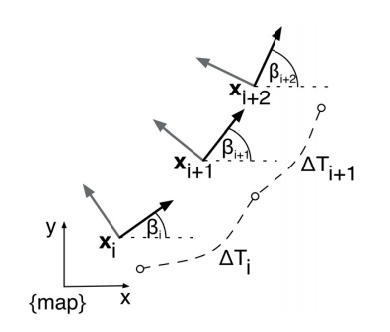
\includegraphics[width=0.3\textwidth]{2.png}
\caption{\label{fig:2}TEB:一组表示机器人的三元组示例}
\end{figure}

这个时候我们可以用一个式子表示这一组三元组的集合.

\begin{equation}
Q = \{ \boldsymbol{x}_i\}_{i=0...n} n\in \mathcal{N} 
\label{equa1-1}
\end{equation}

TEB算法是基于每个三元组状态的时间差来进行计算的,我们这个时候规定$\tau$是每个三元组(帧)的时间差

\begin{equation}
\tau = \{ \Delta T_i\}_{i=0...n-1} n\in \mathcal{N} 
\label{equa1-2}
\end{equation}

每个时间差表示机器人依次从一个配置转换到下一个配置所需的时间.TEB定义为两个序列的元组:

\begin{equation}
B:=(Q,\tau)
\label{equa1-3}
\end{equation}

该算法关键思想是通过实时加权多目标优化,在配置和时间间隔方面调整和优化TEB：我们可以定义一个函数代价函数f,然后我们优化上面提到的B让这个函数f的值最小.

\begin{equation}
f(B) = \sum_k \gamma_kf_k(B)
\label{equa1-4}
\end{equation}

\begin{equation}
B^* = argminf(B)
\label{equa1-5}
\end{equation}

在上面的式子中$B^*$代表已经优化过的TEB.在本文中,它是捕获各个方面的分量fk的加权和.这是多目标优化的最基本方法,但它已经产生了非常好的结果.在未来的工作中,可能会研究更复杂的方法.

目标函数的大部分组成部分是相对于B而言是局部的,因为它们只依赖于少数连续配置的数量,而不是全局的.TEB的这种局部性导致稀疏系统矩阵,专门用于稀疏矩阵的、快速高效的大型数值优化方法都是可用的\cite{11}.

TEB的目标函数分为两类：约束条件,如速度和加速度限制,和轨迹优化目标,如最短或最快路径或与障碍物的间隙.

在自由使用的实现中,稀疏约束优化算法在机器人框架（例如ROS）中不易获得.

因此,在“TEB”的情况下,这些约束被表述为分段连续、可微成本函数,这些函数惩罚违反约束的行为.

我们一般使用下面的惩罚函数:

\begin{equation}
e_{\Gamma}(x,x_j,\epsilon,S,n)=(\dfrac{x-(x_r-\epsilon)}{S})^n\ (x>x_r-\epsilon)
\label{equa1-6}
\end{equation}
其中,$x_r$为极限值,S、n和$\epsilon$影响近似的准确度.具体地说,S表示缩放,n表示多项式阶数,$\epsilon$表示近似值附近一个小位移.x就是输入,这里x和$x_j$是距离.

\begin{figure}[htbp]
\centering
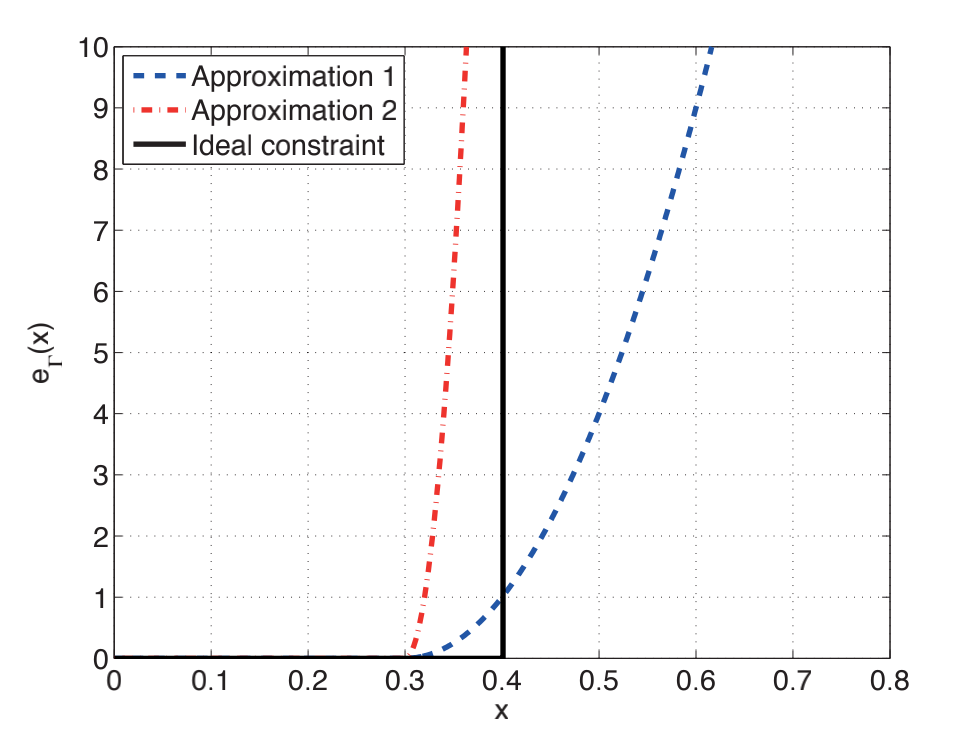
\includegraphics[width=0.5\textwidth]{3.png}
\caption{\label{fig:3}约束的多项式逼近函数图像}
\end{figure}

图\ref{fig:3}显示了等式\label{equa1-6}的两种不同实现.Approximation1由参数集$n=2,S=0.1,\epsilon =0.1$产生,Appro-imation2由参数集$n=2,S=0.05, \epsilon=0.1$产生.该示例显示了约束$x_r=0.4$的近似值.这个可以反应这个数学函数的逼近模式.

使用多目标优化框架的一个明显优点是目标函数的模块化表达.TEB目前采用的目标函数由下面的部分组成.

\subsection{路线点和障碍点}

TEB同时考虑了原始路径的中间路线点的实现以及静态或动态障碍物的避免.这两个目标函数都相似,不同之处在于路点吸引弹性带,而障碍物排斥弹性带.目标函数基于TEB和路点或障碍物$z_j$之间的最小间隔$d_{min},j$（图\ref{fig:4}）.在路点的情况下,距离由最大目标半径$rp_{max}$（等式7）从上方界定,在障碍物的情况下由最小距离$ro_{min}$（等式8）从下方界定.这些约束由等式6中的惩罚函数实现.

假设一个点$A$,当前小车的与这个点的距离设置为$\alpha = |\boldsymbol{x}|$.

$A$是目标点.那么这个函数就是:
\begin{equation}
f_{path} = e_{\Gamma}(\alpha,r_{pmax},\epsilon,S,n)
\label{equa1-7}
\end{equation}

这代表,我们需要让这个小车离这个目标点越来越近.$r_{pmax}$是自己设置的临界值

$A$是障碍点.那么这个函数就是:

\begin{equation}
f_{op} = e_{\Gamma}(-\alpha,-r_{omin},\epsilon,S,n)
\label{equa1-8}
\end{equation}
这代表,我们需要让这个小车离这个目标点越来越远,所以说要加上负数.$r_{omix}$是自己设置的临界值.

\begin{figure}[htbp]
\centering
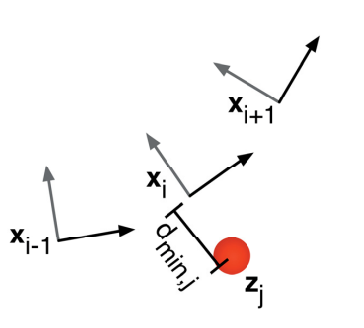
\includegraphics[width=0.3\textwidth]{4.png}
\caption{\label{fig:4}算法躲避障碍点的相关数据示意图}
\end{figure}

\subsection{速度和加速度}

机器人速度和加速度的动态约束与案例中的惩罚函数相似,图\ref{fig:2}显示了TEB的相关规定.平均平移和旋转速度为根据欧氏距离或角距离计算,计算的方式如下:

\begin{equation}
v_i = \dfrac{1}{\Delta T_i}(x_{i+1}-x_i)
\label{equa1-9}
\end{equation}

\begin{equation}
\omega_i = \dfrac{1}{\Delta T_i}(\beta_{i+1}-\beta_i)
\label{equa1-10}
\end{equation}

由于配置的邻近性,欧氏距离是两个连续姿势之间圆形路径的真实长度的充分近似.加速涉及两个连续的平均速度,因此包括三个连续的配置,具有两个对应的时间间隔：

\begin{equation}
a_i = \dfrac{2(v_{i+1}-v_i)}{\Delta T_i+\Delta T_{i+1}}
\label{equa1-11}
\end{equation}

为了清楚起见,我们可以让三种连续配置用方程11中的两个相关速度代替,角加速度的计算也可以使用这个方式来代替.我们在考虑总体的速度的时候还要考虑转动所带来的影响.在此我们可以进行修正:

\begin{equation}
v_{\omega_{R,j}} = v_i + L\omega_{i}
\label{equa1-12}
\end{equation}

\begin{equation}
v_{\omega_{L,j}} = v_i - L\omega_{i}
\label{equa1-13}
\end{equation}

上面的公式中,L是机器人的刚体力学臂长.

关于时间微分方程12和方程13可以计算相应的靠谱加速度.角速度和角加速度的限定根据机器人制造商规范进行制定.这个机器人的平移和旋转惯性可以以一种明显的方式包括在内,但在第一次实现中我们还没有这样做.

\subsection{非完整运动学约束}

\begin{figure}[htbp]
\centering
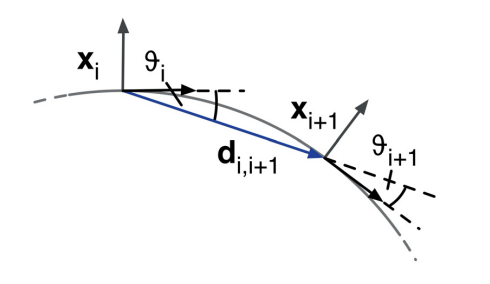
\includegraphics[width=0.5\textwidth]{5.png}
\caption{\label{fig:5}对于非完整运动学圆上配置之间的关系}
\end{figure}

具有差速驱动的机器人只具有两个局部自由度.因此,它们只能执行机器人当前方向的运动.该运动约束导致由弧段组成的平滑路径.因此,如图\ref{fig:5}所示,两个相邻配置必须位于一个常曲率的公共弧上：初始配置$x_i$和方向$d_{i,i+1}$之间的角度$\theta_i$必须等于最终配置$x_{i+1}$处的相应角度$\theta_{i+1}$.如果$\beta_i$表示机器人在第i个配置下的绝对方向角,为了满足两个位置的轨迹是处于同一个圆弧上的,我们必须满足下面的要求:

\begin{equation}
\theta_i = \theta_{i+1}
\label{equa1-14}
\end{equation}

\begin{equation}
\begin{Bmatrix}
   cos\beta_i\\
   sin\beta_i
  \end{Bmatrix}
  \times
  \boldsymbol d_{i,i+1}
  = 
  \boldsymbol d_{i,i+1}
  \times
  \begin{Bmatrix}
   cos\beta_{i+1}\\
   sin\beta_{i+1}
  \end{Bmatrix}
\label{equa1-15}
\end{equation}

我们定义d为

\begin{equation}
\boldsymbol d_{i,i+1}
  =
  \begin{Bmatrix}
   x_{i+1}-x_i\\
   y_{i+1}-y_i
  \end{Bmatrix}
\label{equa1-16}
\end{equation}

对应的惩罚函数是:

\begin{equation}
f(x_i,x_{i+1})=||(\begin{Bmatrix}
   cos\beta_i\\
   sin\beta_i
  \end{Bmatrix}+\begin{Bmatrix}
   cos\beta_{i+1}\\
   sin\beta_{i+1}
  \end{Bmatrix})\times \boldsymbol d_{i,i+1}||^2
\label{equa1-17}
\end{equation}

目标函数惩罚违反此约束的二次误差,目的是让机器人能在比较平整的圆弧上进行运动.

\subsection{最快路径}

以前的“弹性带”方法通过收缩弹性带的内力获得最短路径.由于我们的方法将时间信息视为最短路径的目标,因此我们可以选择将最短路径目标替换为最快路径目标,或者将这些目标组合起来.最快路径的目标很容易通过最小化所有时间差之和的平方来实现.

\begin{equation}
f_k = \sum (\Delta T_i)^2
\label{equa1-18}
\end{equation}

\subsection{超图}

\begin{figure}[htbp]
\centering
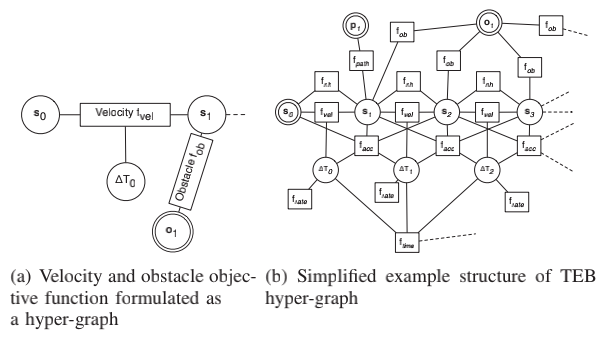
\includegraphics[width=0.5\textwidth]{7.png}
\caption{\label{fig:7}一个示例的超图}
\end{figure}

TEB被定义为标量化的多目标优化问题.大多数所需的目标函数依赖于仅取决于频带的相邻配置的子集的参数：

(1)速度（加速度）约束

(2)与障碍物的间隙和中间航路点的归位影响单个配置及其k个最近邻居（实践中约为3-5）.

(3)遵守机器人的非完整约束涉及两个相邻的配置,这两个配置需要位于恒定曲率的公共弧上.

最快和最短路径是局部结构的例外,因为这些目标全局依赖于所有参数.通过最小化所有时间差之和的平方或时间差平方之和,可以获得具有时间均匀间隔配置的最快路径.

TEB的这种局部性导致了一个稀疏的系统矩阵,该矩阵由超图表示,其中节点对应于配置和时间间隔.包含对同一目标函数有贡献的参数的节点通过相应的多边缘连接.在下文中,方程被转换为超图.超图的定义意味着由单个边连接的节点的数量不限于传统图中的两个节点.超边是传统边的延伸,因为它将多个节点彼此连接起来.每个目标函数取决于TEB状态的子集（配置和时间差）,超边表示目标函数$f_k$,并连接与配置和时间差异相对应的节点,这些节点在其评估中作为参数出现.

图6.a显示了表示与两个后续配置$s_0$、$s_1$、它们的时间差$\Delta T_0$和障碍物$o_1\in R_2$相关的约束和目标的超图的一个简单示例.注意,我们的具体实现将每个配置节点划分为一个位置节点和一个方向节点,以便于目标函数的模块化激活和停用.速度目标函数为机器人能够在分配的时间$\Delta T_0$内行驶的$s_0$和$s_1$之间的距离设定上限.速度多边缘（$f_{vel}$）和加速度多边缘（$f_{acc}$）捕捉动态方面.障碍物与其最近配置（在示例$o_1$和$s_1$中）之间的距离由保证无碰撞路径的最小间隔从下方限定.障碍物位置是根据从机器人架构内的感知层提供的传感器数据推断的.相应的障碍物不进行图形优化,如图6.a中的双圆圈所示.图6.b说明了TEB超图相对于大多数实现的目标函数的更大提取.每个多边缘中的目标函数根据其权重在总体目标函数中表示.除了固定的障碍物节点之外,路点配置p和初始状态$s_0$也是固定的.在我们的应用程序中,我们在控制回路中使用规划器,因此初始状态由机器人的当前配置给出.
\subsection{实现}
图\ref{fig:6}显示了实施TEB的控制流程.在初始化阶段,通过添加默认定时信息,初步增强了初始轨迹的控制效果,以检测符合条件的动态运动.在任何情况下,初始轨迹都是由一个线性段组成的,并有一个旋转,然后进行翻译.因此,在多个多边形之间的演示通常由两个可能的编辑人员提供\cite{9}或者,Reeds Shepp路径可以增强可发射轨道的载荷\cite{10}.

\begin{figure}[htbp]
\centering
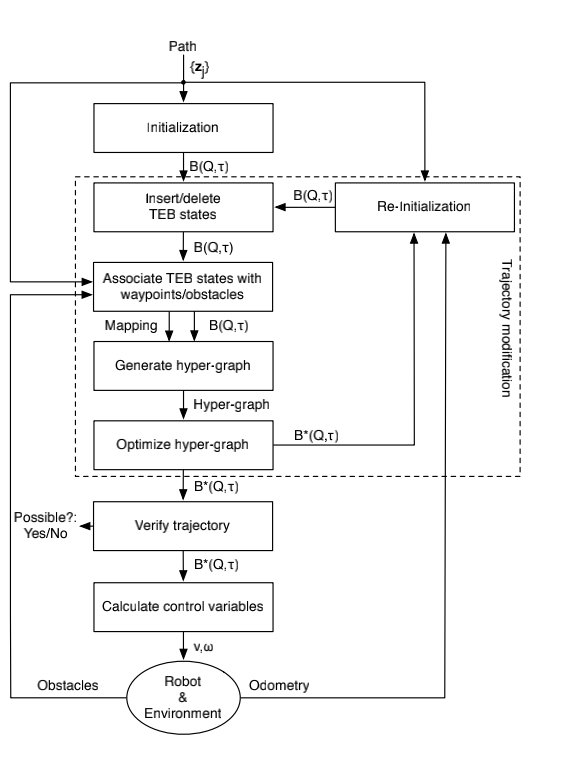
\includegraphics[width=0.5\textwidth]{6.png}
\caption{\label{fig:6}TEB算法实现的控制流}
\end{figure}

在每一次迭代中,算法都会动态地增加或删除新的配置,以调整训练轨迹长度规划范围的空间和时间分辨率.为了避免振荡,实施了一个算法.优化问题被形成为超图,并通过“g2o框架”中的大规模系统切换定时算法来解决\cite{11}.

\section{实验结果}

在这一部份我们简单的给出实验的结果.

\begin{figure}[htbp]
\centering
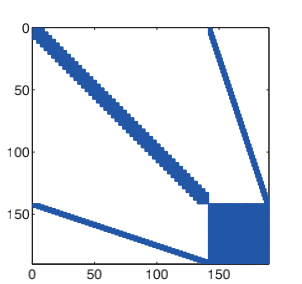
\includegraphics[width=0.5\textwidth]{8.png}
\caption{\label{fig:8}系统矩阵的大小示意图}
\end{figure}

如图8所示,最终的TEB系统矩阵仍然稀疏,有15\%的非零元素.在本示例中,第141个状态响应于状态142-189中的17个状态的时间差$\Delta T_i$.尽管最后一个状态与目标函数相关,目的是实现最快的轨迹,因此,该块随着TEB的尺寸而增大.

\begin{figure}[htbp]
\centering
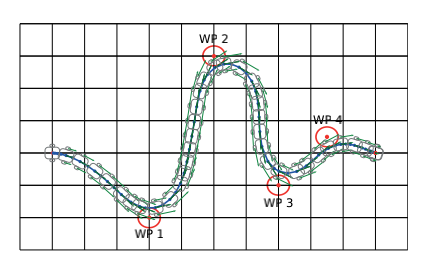
\includegraphics[width=0.5\textwidth]{9.png}
\caption{\label{fig:9}使用约束1的轨迹图}
\end{figure}

\begin{figure}[htbp]
\centering
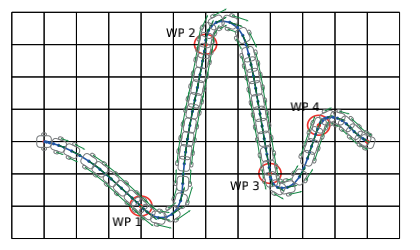
\includegraphics[width=0.5\textwidth]{10.png}
\caption{\label{fig:10}使用约束2的轨迹图}
\end{figure}

图9和图10显示了一个具有四个中间航路点的路线.在这种情况下,根据图3（近似值2）,TEB采用了更为严格的惩罚措施来确定几何参数,因此可以更准确地确定航路点.然而,采用更为严格惩罚措施的解决方案通常会使项目更为顺利,但超调量较小,调整亮度低,以便在更精确或更平滑和更快速的目标之间转换重点.图11和图12的结果展示了才用了动态约束的结果.其中采用约束$v_{max} = 1.4\dfrac{m}{s},a_{max} = 0.4\dfrac{m}{s^2}$的结果如图11所示,采用躲避静态障碍物的结果如图12所示

\begin{figure}[htbp]
\centering
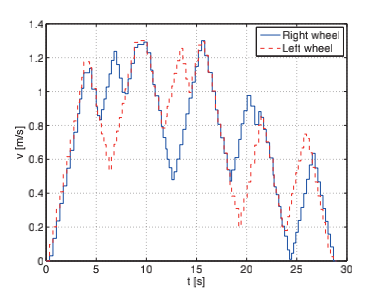
\includegraphics[width=0.5\textwidth]{11.png}
\caption{\label{fig:11}规定了速度限制的左右轮速度图}
\end{figure}

\begin{figure}[htbp]
\centering
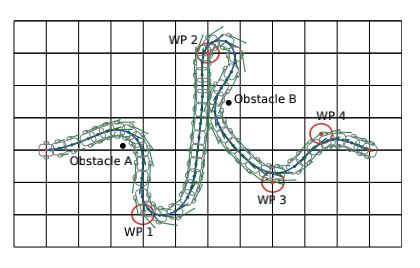
\includegraphics[width=0.5\textwidth]{12.png}
\caption{\label{fig:12}考虑了静态障碍物和中间点}
\end{figure}

用时间信息和备件系统科学规模优化器的可用性增强弹性地带,以实现机器人的实时轨迹适应和控制.

图13显示了与Pioneer2一起拍摄的浪漫实验的顺序.Pioneer3由西门子Lifebooks6410（Core2-Doo,2.4GHz,2GBRAM）控制,并配备了Hokuyo激光扫描仪,以检测物体位置的动态变化.TEBada实时记录了原始的机器人轨迹（t=0）,并在时间间隔$t \in [6,12]$期间避免与人发生任何碰撞,这是一个非常重要的指标.(时间戳是25ms)

\begin{figure}[htbp]
\centering
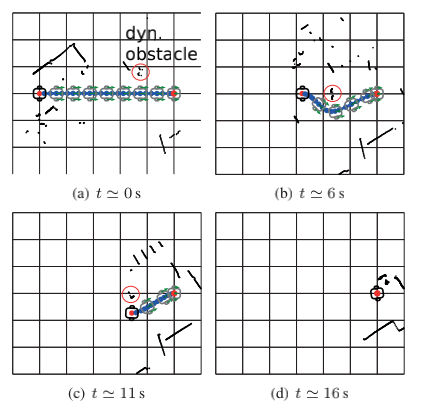
\includegraphics[width=0.5\textwidth]{13.png}
\caption{\label{fig:13}考虑了动态障碍物和中间点}
\end{figure}

\section{总结和展望}
本文提出了一种利用定时弹性带进行实时弹道修正的新方法.它基于时间信息对经典“弹性带”理论的扩充.该方法不仅可以考虑路径上的几何约束,还可以同时考虑移动机器人的动态约束.该算法实时运行,从而直接为下层机器人运动控制器生成命令.该方法高度灵活,易于适应不同的机器人运动学和应用要求.

未来的工作涉及稀疏约束优化框架的开发,从而使当前的惩罚函数约束公式过时.另一个不同的研究方向是使弹性带“跳过障碍物”.从技术上讲,该方法是用一条带围绕一个障碍物,该带的方向比最近点处的轨迹更靠前,将它们粘在切向点上,并在这一点切割产生的轨迹,以获得一条通过另一侧障碍物的轨迹.优化该轨迹后,决定障碍物的哪一侧继续.注意,这仍然是一个局部优化,不能保证找到全局优化.
\bibliography{sample}
\end{document}
